
\documentclass[10.5pt,twocolumn]{article}
\usepackage[utf8]{inputenc}

\usepackage{lipsum} % for dummy text only
\usepackage[pdftex]{graphicx} 
\newcommand{\HRule}{\rule{\linewidth}{0.5mm}} 




\begin{document}

\begin{figure*}[!t]
\centering
\hrule
\vspace{1em}
Department of Electronic \& Computer Engineering \\
Part~{\scshape IV} Research Project Report \\
2014 \\
Refactoring on a Tablet \\
Raoul D'Cunha, Wasiq Kashkari \\
Gerald Weber and Christof Lutteroth
\vspace{1em}
\hrule
\end{figure*}

\clearpage

\begin{figure*}[!t]
\centering
\hrule
\vspace{1em}
Declaration of Originality

This report is my own unaided work and was not copied from nor written in
collaboration with any other person.

\vspace{1em}

Name: Raoul D'Cunha
\vspace{1em}
\hrule
\end{figure*}

\clearpage

\title{Refactoring on a Tablet}
\author{Raoul D'Cunha and Wasiq Kashkari \\
  \multicolumn{1}{p{.7\textwidth}}{\centering\emph{Department of Electrical and Computer Engineering}\\University of Auckland, New Zealand}}
\date{\vspace{-2ex}}
\maketitle

\section{Abstract}
Touch screen based smart tablets have become very popular in the past years and a wide variety of applications have been built, for a wide variety of purposes, for these devices. Programming and refactoring code on a tablet however is very time-consuming and error prone. In this paper we propose a tool named TREAfactor, which supports intuitive touch based refactoring on a tablet device. Users can use touch-based gestures to move, delete and edit text. TREAfactor displays code in a TreeView, which is optimized to take advantage of the screen real estate provided by tablets. 

Code Editing in TREAfactor is powered by our Smart Editing Engine, which can generate context aware editing interfaces based on the code component that the user wants to edit. Auto-complete support has also been implemented, to reduce the number of keystrokes required while typing.  A Usability study conducted on our tool showed that most users felt that TREAfactor had intuitive support for gestures. Refactoring using our tool was not as fast when compared to desktop based IDE’s, however most users felt that it offered significant advantages and improvements over existing tablet-based tools.

\section{Introduction}
Code Refactoring is a process used to improve the quality of a code base. Refactoring involves changing the structure of existing code without causing a change in its external behavior. Code quality is improved with refactoring by enabling non-functional attributes of code. Refactoring can result in improved code readability and reduced complexity in the code base. Maintainability can also be improved by refactoring, by making the code open to modifications in the future.


Refactoring is primarily carried out on Desktop Integrated Development Environments (IDE’s). An IDE normally consists of a source code editor; build automation tools and a debugger. Most modern IDEs offer Intelligent code completion features and advanced refactoring support. Microsoft Visual Studio and Eclipse are two of the most commonly used IDE’s used for writing and refactoring code. Refactoring on these IDE’s is primarily carried out through the use of a Mouse and a Keyboard.


The rising popularity of smart based devices in the recent years has heralded a paradigm shift in computing. The availability and rising computational power of these devices has resulted in these devices being used as potential successors for desktop and laptop computers. It is estimated that 1 in every 5 people in the world own a smart device \cite{Bus}. The Android Operating System is one of the most widely used operating system on these devices, with approximately 81\% of the market share. 


Tablet devices provide the users with a much larger display than smart phone devices. The size and portability of these devices has resulted in users using them for web browsing and basic document editing. Input on these devices is usually provided through either stylus and/or touch gesture recognition. Due to the repositioning and structural nature of refactoring, we felt that these devices would serve as a host to intuitive touch based refactoring tools.


Code editing and refactoring on a tablet-based environment is a problem that has been addressed before. Various IDE’s and tools exist on the Google Play Store that support the editing and development of code, such as \cite{aide}. However, most of these tools try to model their User Interface on existing desktop-based IDE’s, resulting in presentation of a poor, unintuitive User Interface to the user. Most of these tools present code in a text-based viewer, which poses a problem on touch screen devices, because typing is very hard on a tablet \cite{Lu:2012:GCT:2207676.2208693}. These tools also have minimal support for gestures resulting in a poor experience for the user.


In this paper, we explore the idea of using a tree-based user interface for displaying and editing code, with support for gesture based refactoring. We present a novel tool name TREAfactor, which leverages both the touch screen nature of tablets and limited screen estate (when compared to traditional desktop and laptop computers) to provide an effective refactoring tool to the user. We address the following research questions:

\begin{itemize}
    \item [\textbf{R1}] Is Gesture based refactoring usable?
    \item [\textbf{R2}] Can we leverage the touch-based nature of a tablet to provide an efficient mechanism for gesture based refactoring?
    \item [\textbf{R3}] How effective would this tool be, when compared to traditional refactoring tools in terms of the time it takes a user to refactor code?
\end{itemize}

We conducted a user study to evaluate the usability and effectiveness of our TREAfactor proof of concept prototype and address our research questions. This evaluation was fairly small in scale and scope, but was novel due to the fact that there is very little prior research done on touch based refactoring support on touch screen devices. Most of the prior research done was focused on display and editing of code on desktop based devices using a mouse or stylus.

Section 3 gives and overview of related work done on this topic. Section 4 summarized the requirements for developing a touch based refactoring tool on the tablet. Section 5 introduces TREAfactor and discusses it's design while Section 6 covers the implementation of the tool. Section 7 describes the evaluation conducted by the tool and the results gathered from the study. Section 8 proposes future work that can be undertaken on both the tool and this topic, while Section 9 concludes the paper.


\section{Related Work}
Scratch \cite{Resnick:2009:SP:1592761.1592779} is a graphical programming language and programming environment developed for kids at the Massachusetts Institute of Technology.  Puzzle-piece shaped “blocks” are used to create code in Scratch.  These blocks represent and provide functionality, such as variables, lists and events and can connect with each other like a jigsaw puzzle. Each block has its own shape and a specially shaped slot for it to be inserted into, to prevent syntax errors.

Programming in Scratch can be done without requiring a lot of keyboard input, as the user interface is very drag and drop orientated. The blocks can be freely moved around the screen, as long as they are follow the slot insertion constraint, and hence it is an excellent model for touch based programming and refactoring development environments. 

Some of the drawbacks of Scratch are that it provides an abstract visual representation of code and provides no way to view lower level implementation details of the code. There is also no support for common refactoring methods, such as renaming variables, and hence the user must carry this out manually.

Android IDE (AIDE) supports the development of Android, Java and PhoneGap Applications on an Android device \cite{aide}. It consists of a text editor that has basic support for code editing and refactoring. Auto-completion is provided during code editing for “for” and “while” loops and also for method and variable names.  The interface provided by AIDE however, is not really optimized for touch screen input. 

There is no support for moving blocks of code around the page, and most of the settings and refactoring tools are hidden behind drop down menus. The refactoring tools, such as ‘Method Rename’, work well, but provide no feedback or visual cues, about the affected lines of code, when used. 

Code Bubbles \cite{codeBB} is an IDE that is based upon collections of code fragments called bubbles, which are grouped together to form concurrently visible working sets. This bubble-based representation provides an intuitive visualization of the interaction of objects and their dependencies to the developer. While this bubble based representation translates well to touch based input, the IDE does not provide much refactoring support and the use of a keyboard is necessary for most refactoring operations.

\section{Requirements}
A successful execution of this research endeavor should meet the following requirements:
\begin{enumerate}
\item The development of a refactoring tool developed for the Android platform.
\item The user interface of the IDE will be designed for an Android tablet device and hence will have to aptly use all the limited screen real estate provided by these devices.
\item Support for common refactoring methods, such as module restructuring, method and class extraction and the introduction and removal of intermediate variables.
\item Support for gestures and other touch-based interactions that are both intuitive and natural on tablet environment that aligns with a user’s mental model. This would require the minimization of keyboard based input and usage, as typing in these environments are time consuming and error prone.
\item The IDE should be extensible for future improvement and development, as only a subset of the refactoring methods will be implemented.
\item Evaluation on the usability of the IDE, when compared with existing Android IDEs.
\end{enumerate}

\begin{figure}[h]
    \centering
    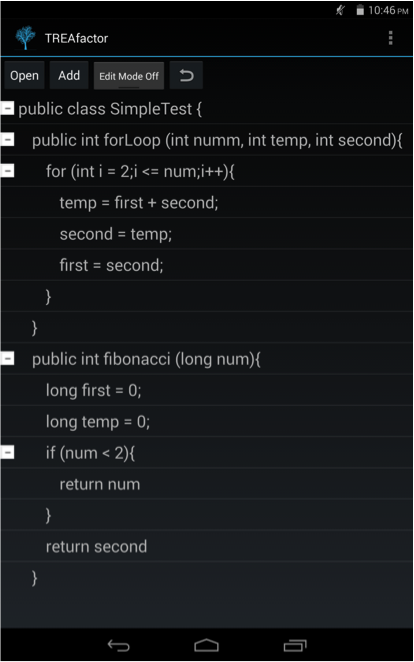
\includegraphics[width=0.25\textwidth]{screenshot}
    \caption{TREAfactor User Interface}
    \label{fig:tf1}
\end{figure}
\section{Design}


TREAfactor displays a tree based user interface for displaying and editing code. It supports natural gesture based interactions for common operations. Code can be restructured and moved around though dragging and dropping blocks and lines. Code can also be deleted by swiping away code lines.

We have also developed a Smart Editing Engine that is used in TREAfactor to create and edit code. This engine supports the creation of common code elements such as methods, statements and variables. Context sensitive code editing, facilitated by the Smart Editing Engine is also implemented in the tool.


\begin{figure}[h]
    \centering
    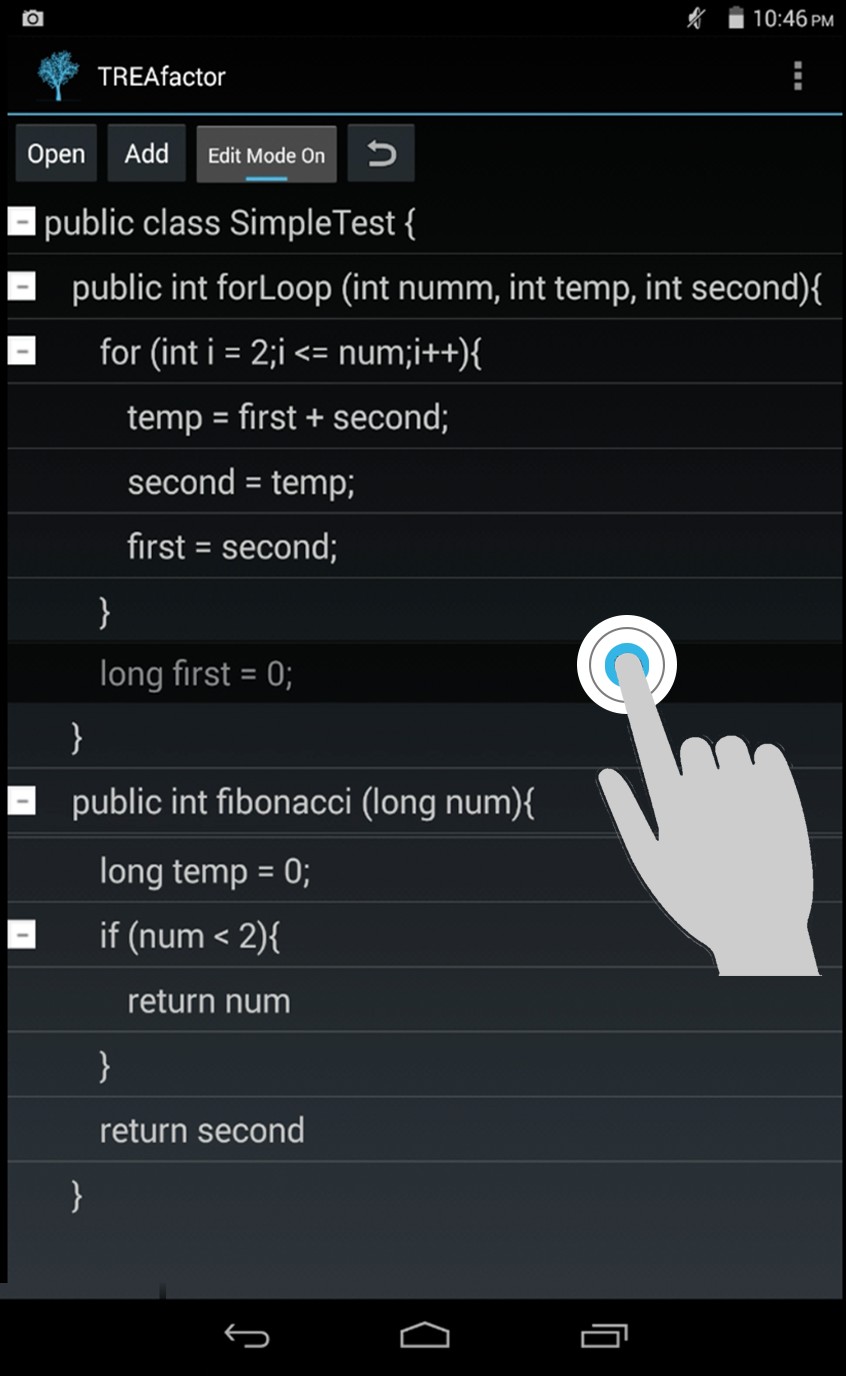
\includegraphics[width=0.25\textwidth]{taptomove}
    \caption{Lines can be tapped and dragged to be moved}
    \label{fig:tf6}
\end{figure}

The User Interface of TREAfactor consists primarily of a TreeView with a menu bar on top, as shown in Figure \ref{fig:tf1}. The menu bar has buttons for common operations such as opening a log file and adding new code elements to the code. The tool initially displays code in a read only TreeView. Toggling the Edit Mode switch enables editing and refactoring functionality in the TreeView such as swipe to delete, tap to edit and drag to move.

The decision to use a TreeView to display code provided us with various advantages when compared to traditional text based views. Code is inherently hierarchical in nature. Classes contain methods, methods contain declarations, statements and other expressions. This means that using a text based view to represent code, especially on a smaller screen size would result in poor utilization of the real estate provided by the screen. A TreeView provides a way to display and view hierarchical data in a structured manner. It is also possible to collapse and expand nodes in a TreeView, making it ideal for tablet devices, as information can be hidden and shown on demand to reduce screen clutter. Due to these reasons, we decided to display code in a TreeView in TREAfactor.

\begin{figure}[h]
    \centering
    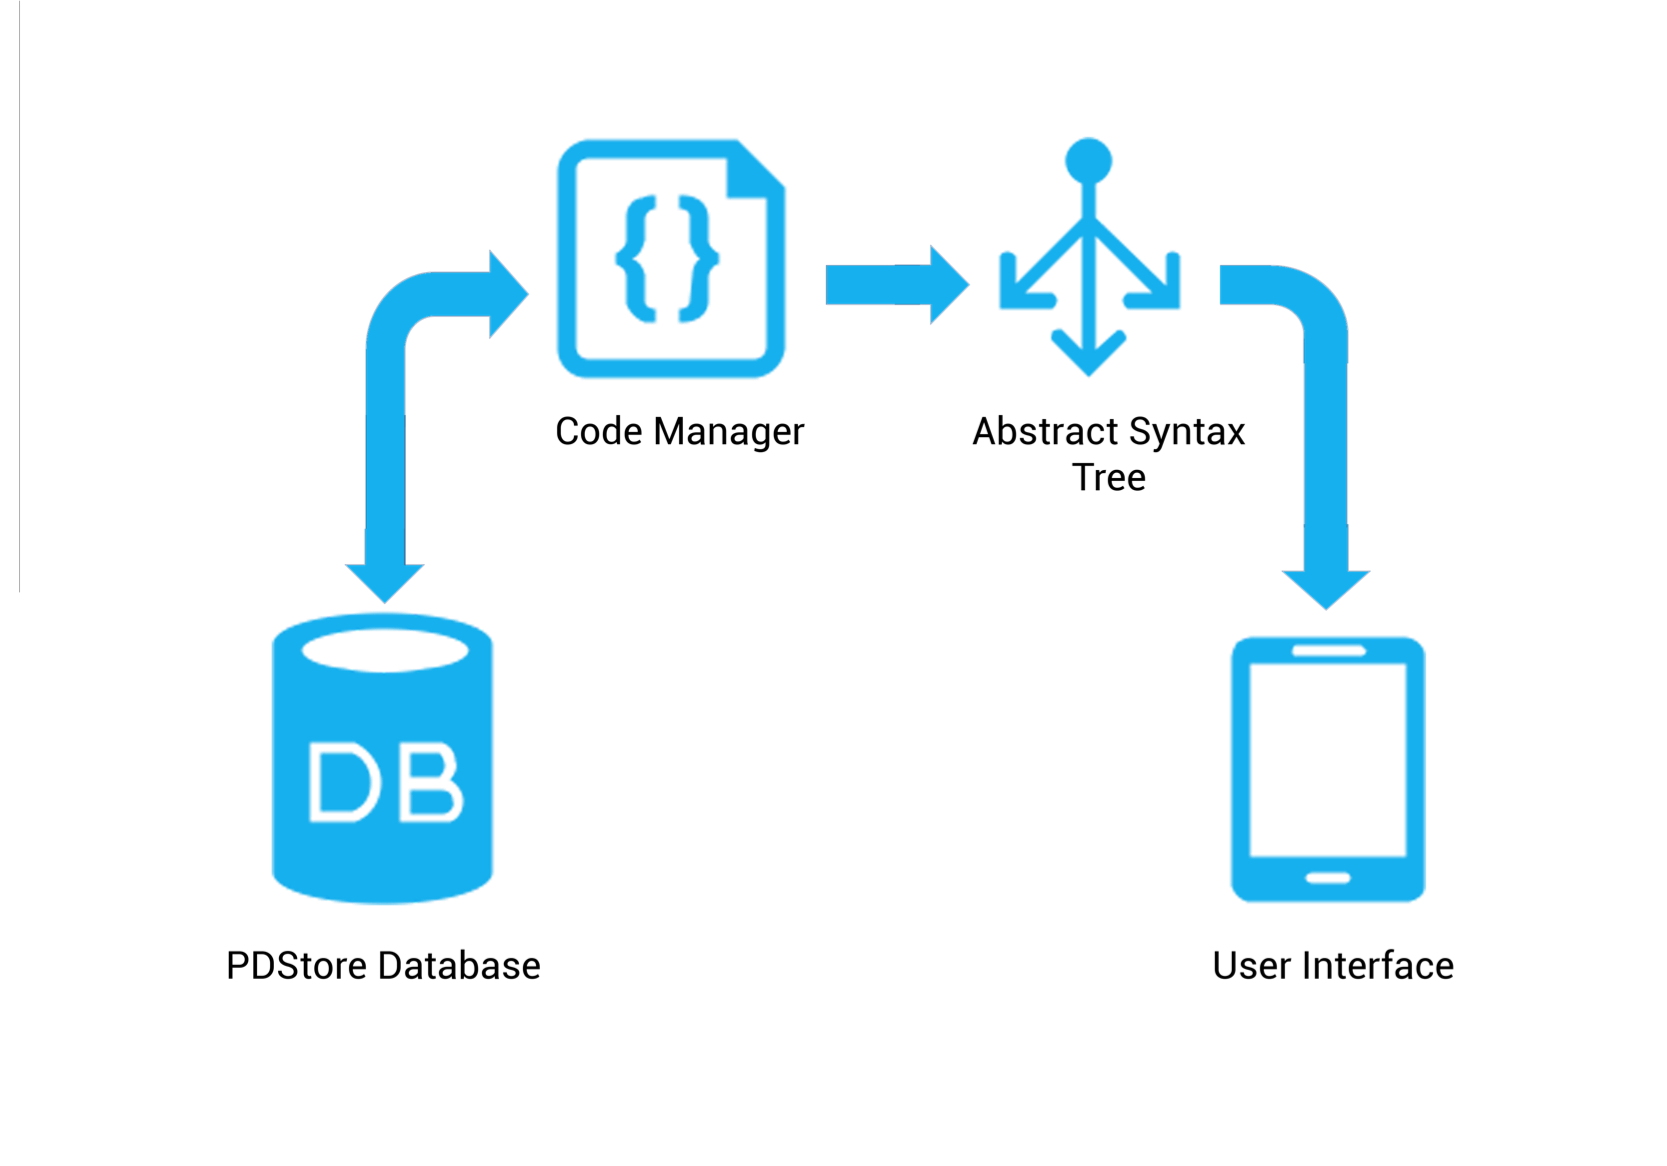
\includegraphics[width=0.5\textwidth]{architecture}
    \caption{TREAfactor Architecture}
    \label{fig:tf2}
\end{figure}

The design of TREAfactor is composed primarily of the four key components displayed in Figure {fig:tf2}. The four main components are the PDStore Database, Code Manager, Abstract Syntax Tree and the User Interface. We decided to split the design and base TREAfactor on these components because it allowed us to easily perform separation-of-concerns so as to separate the data from the data processing and the User Interface.  


\section{Implementation}
The Implementation of the tool was done in Java and was targeted towards SDK 19 of the Android Platform. The implementation of each of the four components of TREAfactor is described below

\subsection{PDStore Database}
The PDStore Database is a triple store database developed at the University of Auckland \cite{PDS}. A partial port of this database existed on the Android Platform, and we worked on and completed the port, to use it in our tool. Data in a triple store database is represented as objects and roles between objects. This structure enables us to store code, represented as an Abstract Syntax Tree directly into the database without any modifications. 

Supporting the importation of code into the database and generation of an Abstract Syntax Tree representation of that code was beyond the scope of this project, as that functionality is already supported by the PSImporter plugin for the IntelliJ IDEA IDE. The exportation of the refactored code is also beyond the scope of this project as this functionality is also provided by a similarly named PSIExporter plugin. 

\subsection{Code Manager and Smart Editing Engine}
The Code Manager is responsible for communication between the Database and the User Interface. It queries the Abstract Syntax Tree stored in the database to generate objects that are then passed to the Abstract Syntax Tree Module. The manager exposes various methods that can be used by the User Interface and Abstract Syntax Tree module to query statements imported by the PSImporter tool into the PDStore database.

The Smart Editing Engine is responsible for the Context aware editing support provided by the tool. This functionality is possible due to the ability of each code line to edit itself. The editing capability is provided by the Node interface, which is implemented by each code component. The implementation of this method in the concrete classes such as Variable and Method allow the definition and creation of a custom Android UI component, which displays editable parameters on the screen.

\subsection{Abstract Syntax Tree}
The Abstract Syntax Tree Module is responsible for generating an in-memory Abstract Syntax Tree (AST).  An AST is a data structure that is designed to store code in memory. The nodes of the tree usually contain an operator as a parent and operands as children. This in-memory AST is easily query-able for code components and is also easily editable.

\subsection{TreeView}
The TreeView module is responsible for displaying the Abstract Syntax Tree of the code in a TreeView view on the tablet. Android does not support for a built in TreeView control and hence we had to implement one from scratch. Our initial efforts resulted in creating a TreeView based on the ListView control on Android. However this approach proved to be complicated and we decided to use an existing Android TreeView library, which also allowed us to implement additional functionality easily. Tree-View-List-Android was then implemented as the TreeView for our tool. This library was also based on the ListView control of the platform.

Touch based gesture support was implemented by using the DragSortListView library. This library is an extension of the Android ListView that enables drag-and-drop reordering of list items. Gestures such as drag to move, tap to edit and swipe to remove were implemented by using this library as a base.



\section{Evaluation}

An evaluative study was carried out to assess the usability of the tool. The purpose of this study was to address our research questions and find out if TREAfactor met all the requirements that we proposed for a touch based refactoring tool.

\subsection{Methodology}
The user study was conducted by making the participants carry out tasks on both TREAfactor and Eclipse and recording the completion time for each task. Data was gathered both during and after the completion of the tasks using the various approaches described below:

\begin{description}
    \item [Observations:] The participants were observed while completing the tasks and any notable observations were noted down.
    \item [Thinking aloud:] The participants were encourage to think aloud, so as to enable us to understand their thought processes with respect to the tool, and hence identify key issues and problems with the tool.
    \item [Questionnaire:] The questionnaire handed out to the participants at the end of the study included a combination of Likert scale questions and open-ended questions. The Likert scale questions allowed us to evaluate specific functionality of TREAfactor, while the open-ended questions were used to gather feedback from the users while also asking them about their likes and dislikes. The questionnaire consisted of 12 Likert questions and 4 open-ended questions.
\end{description}

The participants were asked to conduct two tasks on both TREAfactor and Eclipse. The tasks are listed below:

\begin{enumerate}
  \item Perform some refactoring operations on a class
  \item Create simple new methods in an existing class
\end{enumerate}

This first task consisted of refactoring a simple iterative Fibonacci sequence generator. Refactoring tasks consisted of extracting structured code blocks into new methods and introducing new intermediate variables.  Users were also required to re implement while loops as for loops. This showcased the Smart Edit Engines ability to create context sensitive interfaces could reduce time taken during refactoring in certain situations.


The second task required the participants to create simple methods, one to calculate the area of a circle after being provided its radius and the other to calculate multiple areas after being given multiple radii. This task was used to demonstrate TREAfactors ability to write code in a tablet environment.


The tasks were individually timed, for both TREAfactor and Eclipse. A maximum time of 10 minutes was allocated towards each task. If a participant failed to complete a task in the allocated time, we intended to walk through the task along with the participant and identify any key issues or challenges that they faced that prohibited them from completing the task. However, all the participants finished all the tasks well before the allocated time, so we did not do the walkthrough with any participant.

Training was also provided to the participants at the start of the session. This was done by briefing them about the tool and giving them an overview of all the key features and functionality of TREAfactor. We also ensured that the participants were familiar with the refactoring tools provided in Eclipse, so as to ensure that all participants were familiar with both the tools.

\subsection{Results and Discussion}
The study was undertaken on 7 participants, of intermediate to advanced programming skills. All participants were Software Engineering students at the University of Auckland and had prior experience with respect to refactoring code. Most of the participants had experience with multiple desktop-based IDE’s, with the most popular ones being Microsoft Visual Studio and Eclipse. 4 out of the 7 participants had prior experience with programming and refactoring on a tablet based environment.

\begin{figure}
    \centering
    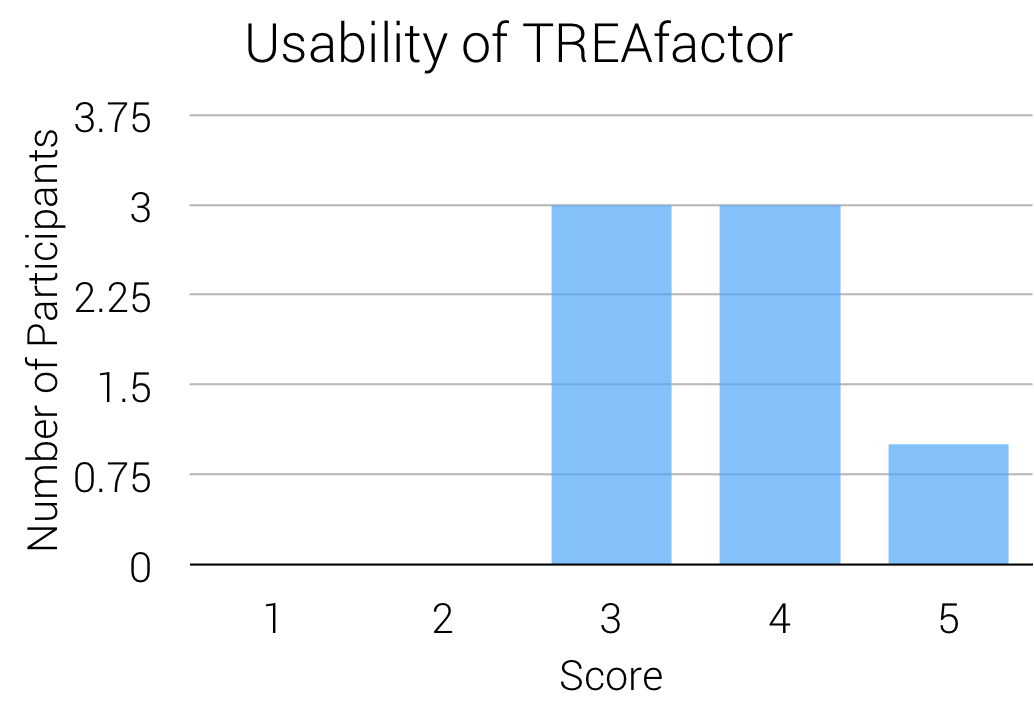
\includegraphics[width=0.5\textwidth]{tfusability}
    \caption{Usability of TREAfactor}
    \label{fig:tf4}
\end{figure}

\begin{figure}
    \centering
    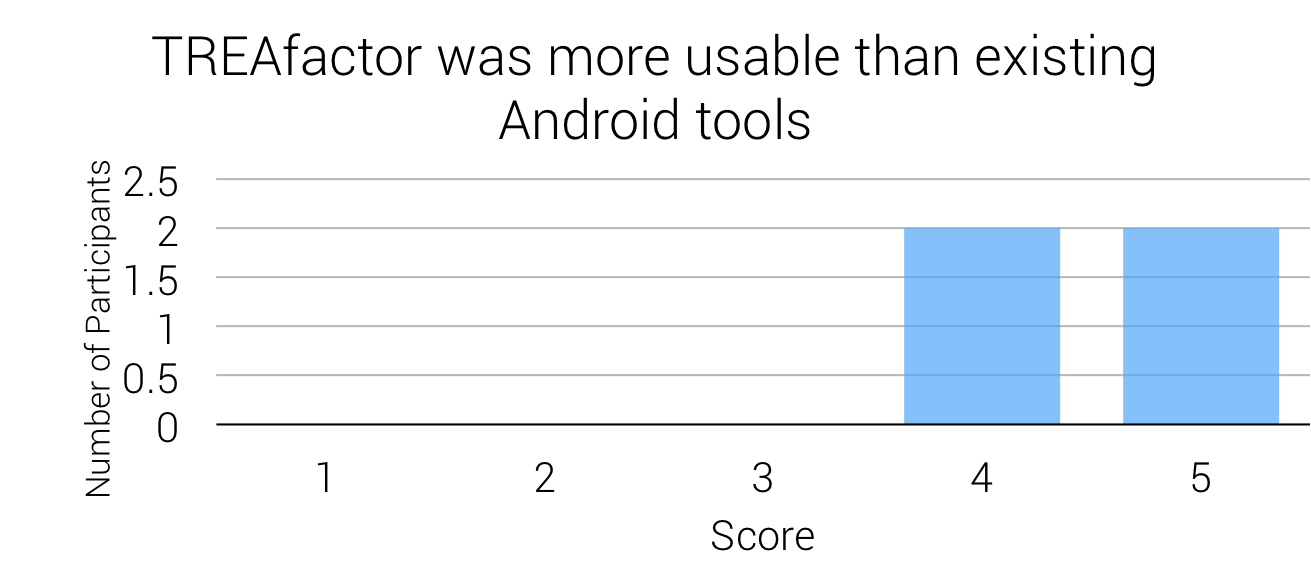
\includegraphics[width=0.5\textwidth]{tfvsandroid}
    \caption{User ratings of TREAfactor usability when compared to existing Android tools}
    \label{fig:tf5}
\end{figure}

The results of the study were generally positive. Overall, the participants rated the tool favorably with most participants rating TREAfactor a 4 or higher on the Likert scale as shown in Figure \ref{fig:tf4}. The participants also found TREAfactor’s Gesture support to be intuitive and usable. However, the participants took a significantly longer amount of time to complete both the tasks on TREAfactor than on Eclipse. Figure \ref{fig:tf3} shows that it took the participants a combined time of averaging around 6 minutes on Eclipse, while it took them on average 10 minutes each to complete the same tasks on TREAfactor. Participants with prior experience with regards to refactoring on a tablet did however state that TREAfactor was a much more usable tool than existing tablet based tools. These participants rated TREAfactor a 4 or higher, as shown in Figure \ref{fig:tf5}.

\begin{figure}
    \centering
    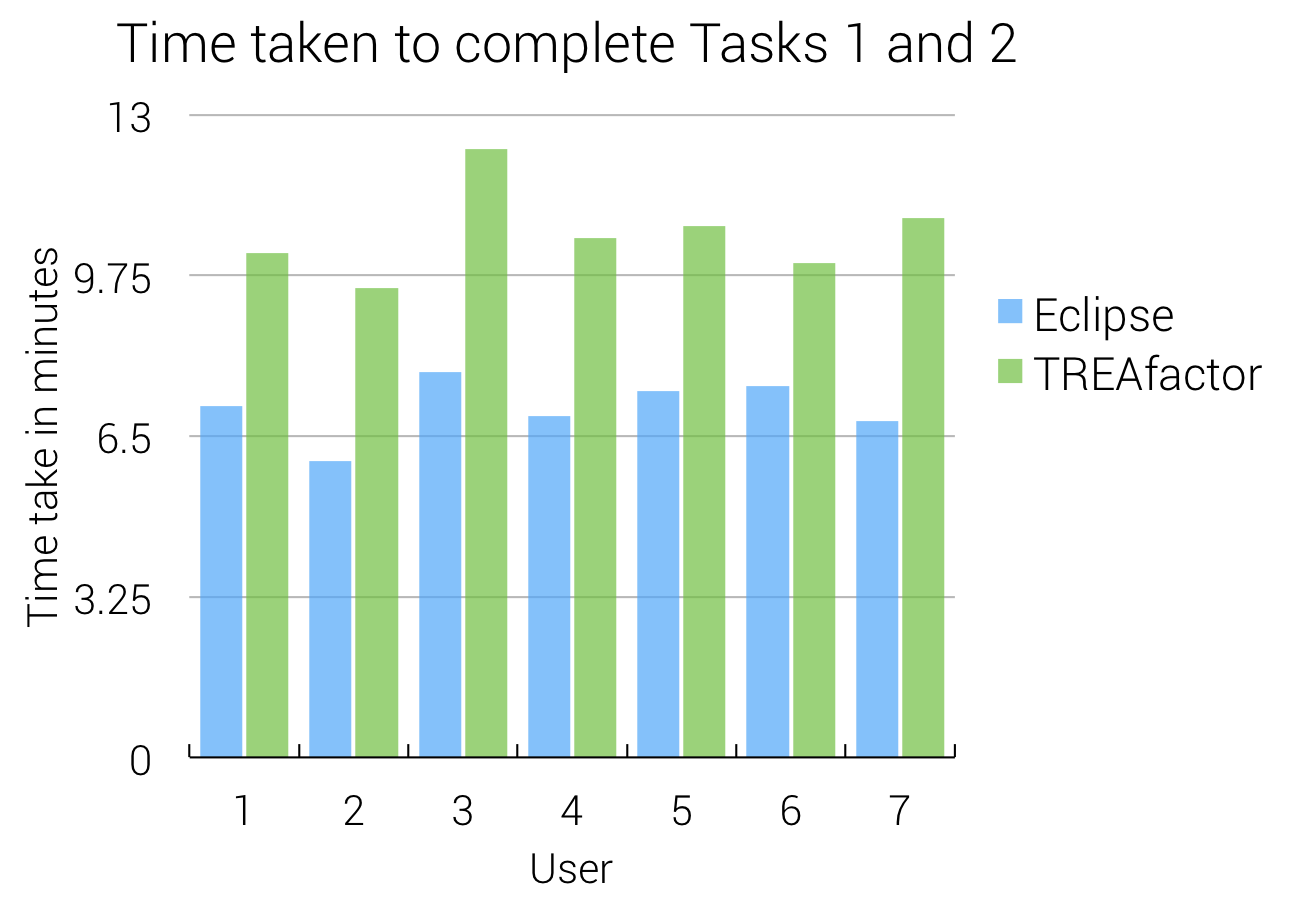
\includegraphics[width=0.5\textwidth]{timefortasks}
    \caption{Time taken to complete Tasks 1 and 2}
    \label{fig:tf3}
\end{figure}

The difference in time between refactoring on TREAfactor when compared to Eclipse could be due to a wide variety of reasons. Participants in general had spent a much longer time working on desktop-based IDE’s in the past. Most of the participants were intimately familiar with the tools and options provided by Eclipse. Performing certain operations with a mouse and keyboard is also significantly quicker than performing the same gestures using touch gestures, when the participant is much more familiar and comfortable with a mouse and keyboard. The time difference between TREAfactor and Eclipse could be improved by adding support for additional multi-finger gestures to select and swipe away multiple blocks of code, which is slower on TREAfactor than on Eclipse.

Feedback gathered from the participants indicated that they wanted to see Syntax Highlighting support in the tool. Some of the participants said that they would like the ability to see more than one class at once - perhaps in a split or a tabbed view. Participants also wanted multi-finger gesture support in the tool and they wanted support for styluses and other input devices.

The small sample size is one of the limitations of our study. It has been shown however that small sample sizes are generally acceptable for qualitative usability studies, as potential problems can easily be identified even with a few participants \cite{faulkner}. We tried to increase familiarity with the tool by conducting a training session before starting the tasks, however a study should also be conducted to evaluate the usability of the tool once candidates have spent a significant amount of time playing around with it. A study with a larger sample size must also be conducted on professional programmers, to further gauge the usability of the tool. A evaluation should also be undertaken between existing tools on tablet devices and TREAfactor, to accurately gauge how usable it is when compared with these tools.

\section{Future Work}
Recommendations for future work can be split into improvements on three categories: The User Interface of the tool, The Code Manager and Smart Editing Engine and the Database.

There are various improvements that can be carried out on the User Interface of the tool. Improvements could be made to the Auto-complete suggestions that are provided by the tool, to make them context aware. This improvement could be carried out by adding support for auto-complete suggestions to the Smart Editing Engine, which can provide context based suggestions. Syntax highlighting support would also be a useful improvement to the tool and it would significantly improve user experience. Adding support for multi-finger gestures and styluses would further improve the usability of the tool, along with the ability to view more than one class at once.

Improvements to the Code Manager and the Smart Editing engine would add new functionality to the tool. Support for advanced language features such as Lambda Expressions could be added in the engine. The usefulness of the tool would also be significantly improved if the engine was made language independent, instead of just targeting Java as it currently does. Adding an undo stack for undo operations would significantly improve the usability of the tool and will grant the users the ability to recover from errors and mistakes.

Improvements to the database are mainly out of the scope of this project. However functionality can be added to enable exportation of the in-memory AST to the database. This would enable users to save the changes that they make on the code.


\section{Conclusion}

In this paper we have proposed an intuitive touch based refactoring tool named TREAfactor, that attempts to address the issue of refactoring code on a tablet. We proposed three research problems that we attempted to answer by evaluating our tool.We showed how the limited screen real estate, provided by tablet devices, can be effectively utilised to display and represent code.

The Usability Study conducted on our tool shows that Gesture based refactoring can be intuitive and usable on a tablet device. While the tool was not as effective as traditional desktop based IDE's, the participants of the study felt that it offered a significant improvement over existing tablet tools.

The Usability study also showed that improvements could be made to both the functionality and the usability of the tool. Further studies and research could be guided towards the implementation and usefulness of multi-touch gestures for advanced refactoring operations. For now, the TREAfactor tool offers a promising first step towards touch gesture based refactoring on a tablet.

\section{Acknowledgements}
I would like to graciously thank my project supervisors Gerald Weber and Christof Lutteroth for their guidance and support. I would also like to thank my project partner Wasiq Kashkari for his help with the project.

\bibliographystyle{plain}
\bibliography{myBib}

\end{document}

